\documentclass[conference]{IEEEtran}
\IEEEoverridecommandlockouts

\usepackage{cite}
\usepackage{amsmath,amssymb,amsfonts}
\usepackage{algorithmic}
\usepackage{graphicx}
\usepackage{textcomp}
\usepackage{xcolor}

\def\BibTeX{{\rm B\kern-.05em{\sc i\kern-.025em b\kern-.08em
T\kern-.1667em\lower.7ex\hbox{E}\kern-.125emX}}}

\begin{document}

\title{Multimodal Fusion with Adaptive Drift Detection for Social Media Deepfake Detection}

\author{
\IEEEauthorblockN{Aishwarya Sujan}
\IEEEauthorblockA{
\textit{Department of Computer Science and Engineering}\\
\textit{CMR Institute of Technology}\\
Bengaluru, India\\
aiai23cs@cmrit.ac.in}
\and
\IEEEauthorblockN{Dereddy Abhilash Reddy}
\IEEEauthorblockA{
\textit{Department of Computer Science and Engineering}\\
\textit{CMR Institute of Technology}\\
Bengaluru, India\\
dere23cs@cmrit.ac.in}
\and
\IEEEauthorblockN{Gaury Shibu Sanker}
\IEEEauthorblockA{
\textit{Department of Computer Science and Engineering}\\
\textit{CMR Institute of Technology}\\
Bengaluru, India\\
gasa23cs@cmrit.ac.in}
}

\maketitle

\begin{abstract}
Deepfake content on social media is becoming increasingly difficult to distinguish from authentic media as generative models produce realistic video and audio. Existing detection methods often focus on a single modality and can lose reliability when manipulation techniques or media distributions change. This work presents Social Detect, a multimodal application built around the MFAD-Net design. The framework combines visual, frequency-domain, audio, and social-media metadata information for media authenticity analysis. Its implemented image branch uses an EfficientNet-B0 backbone with an FFT-based frequency branch, while the MFAD-Net prototype includes visual, audio, metadata, cross-modal fusion, and feature-drift components. The application is integrated with a FastAPI backend, a dashboard, and a browser extension for analyzing uploaded or rendered social-media media. The evaluation uses accuracy, precision, recall, F1-score, and ROC-AUC where measurements are available, with additional placeholders for filtered-image, audio, multimodal, and drift experiments.
\end{abstract}

\begin{IEEEkeywords}
deepfake detection, multimodal fusion, frequency-domain analysis, social media, distribution shift, deep learning
\end{IEEEkeywords}

\section{Introduction}

The rapid growth of generative artificial intelligence has made it possible to create highly realistic manipulated images, videos, and audio. Such synthetic media, commonly referred to as deepfakes, can be used to alter facial appearance, speech, and other characteristics of genuine content. Their increasing presence on social-media platforms creates concerns related to misinformation, identity misuse, privacy, and digital trust. The rapid sharing of social-media content further increases the difficulty of identifying manipulated media before it reaches a large audience.

Existing deepfake detection methods have primarily focused on individual forms of evidence such as spatial artifacts, temporal inconsistencies, frequency-domain patterns, or audio characteristics. Although these approaches can achieve strong results under controlled conditions, their performance may decrease when content is compressed, transformed by social-media platforms, or generated using manipulation techniques that differ from those present in the training data. In addition, treating visual, audio, and contextual information independently can prevent a detector from exploiting complementary evidence available across modalities.

This work presents Social Detect as an application of the MFAD-Net design for social-media content. The implemented system combines a trained spatial-frequency image branch with heuristic temporal, metadata, compression, noise, and audio signals, while the MFAD-Net research prototype provides multimodal feature extraction, cross-modal fusion, and drift-monitoring components. The image branch currently uses EfficientNet-B0 with an FFT-based branch. The audio pipeline currently includes a dependency-light synthetic-speech detector and an ASVspoof 5-compatible learned-audio training path. ASVspoof 5 is the selected target corpus for the real audio branch, but an ASVspoof-trained checkpoint is not included in the reported results. A detector registry and score-fusion layer allow these components to operate together while preserving modality-specific results.

The remainder of this paper is organized as follows. Section II discusses existing research on deepfake detection, including spatial-frequency analysis, audio-visual detection, multimodal approaches, and generalization. Section III presents the proposed MFAD-Net methodology and its major modules. Section IV describes the system implementation and workflow. Section V discusses the experimental methodology and evaluation protocol. Section VI presents the results and discussion. Section VII describes the limitations and future work, followed by the conclusion and references.

\section{Related Work}

Deepfake detection has been studied using visual, temporal, frequency-domain, audio, and multimodal information. Early approaches largely focused on visual artifacts produced during face manipulation, while later studies explored spectral characteristics that may remain hidden in the spatial representation. Kou \textit{et al.} proposed SFIAD, which combines spatial and frequency-domain features for deepfake detection and evaluates the approach across multiple datasets \cite{sfiad}. This work demonstrates that frequency information can provide complementary evidence to conventional visual features. However, visual-frequency approaches primarily depend on the media itself and do not directly exploit information from other available modalities.

Audio-visual analysis has also emerged as an important direction because manipulated videos may contain inconsistencies between facial movements and corresponding speech. Javed \textit{et al.} investigated audio-visual synchronization and lip movement characteristics for real-time deepfake detection \cite{javed2025av}. Such methods demonstrate the value of combining visual and audio evidence instead of relying on a single stream. At the same time, multimodal deepfake detection introduces additional challenges because different modalities may vary in quality, availability, and reliability. Recent research surveys identify multimodal fusion, robustness, real-time processing, and generalization as important continuing challenges in practical deepfake detection systems \cite{multimedia_survey_2025,multimodal_forgery_review_2025}.

Another important issue is the ability of a detector to generalize beyond the data used during training. Changes in manipulation methods, datasets, compression, and media sources can create distribution differences between training and deployment environments. Recent work on deepfake detection has therefore examined robustness and generalization under changing data distributions \cite{generalization_survey_2026}. Continual-learning research has additionally explored how a detector can learn new manipulation patterns while retaining previously acquired knowledge. Zhang \textit{et al.} proposed a generalization-preserved learning approach for continual deepfake detection to address this adaptation problem \cite{zhang2025continual}.

The existing literature establishes the importance of spatial-frequency information, audio-visual relationships, multimodal fusion, and adaptation to changing distributions. However, these aspects are commonly investigated as separate components. MFAD-Net brings these ideas together by combining visual, frequency, audio, and contextual metadata representations through a common fusion stage and by incorporating distribution-shift monitoring through the proposed Temporal-Semantic Drift Detector. The objective is to provide a modular framework suitable for investigating deepfake detection under the changing conditions encountered in social-media environments.

\section{Proposed Methodology}

MFAD-Net is designed as a multimodal framework for detecting manipulated social-media media by combining complementary information from visual, frequency, audio, and contextual sources. The methodology is divided into four modules: multimodal feature extraction, cross-modal feature fusion, temporal-semantic drift detection, and classification with system integration. The modular structure allows the individual components to be developed and evaluated independently while forming a common detection pipeline.

\subsection{Module 1: Multimodal Feature Extraction}

The first module extracts complementary representations from the available media streams. For video input, the implemented backend uniformly samples frames and applies the image branch to those frames. The application also contains an optional face-region branch based on OpenCV Haar-cascade detection. The current image preprocessing resizes inputs to $224 \times 224$ pixels after an early maximum-dimension downscale, which is also used to reduce the mismatch between training and deployment images. EfficientNet-B0 is used to obtain spatial visual features.

A parallel frequency branch applies the Fast Fourier Transform (FFT) to the processed image. For an input image $I(x,y)$, its two-dimensional Fourier transform is given by

\begin{equation}
F(u,v)=
\sum_{x=0}^{M-1}
\sum_{y=0}^{N-1}
I(x,y)e^{-j2\pi
\left(\frac{ux}{M}+\frac{vy}{N}\right)}.
\end{equation}

The magnitude spectrum is calculated as

\begin{equation}
S(u,v)=|F(u,v)|.
\end{equation}

The spatial and frequency representations are combined to form the visual representation:

\begin{equation}
F_V=[F_{\mathrm{spatial}}\;||\;F_{\mathrm{frequency}}],
\end{equation}

where $||$ denotes feature concatenation.

The audio stream is extracted from the input media and resampled to 16 kHz. The current application uses a dependency-light synthetic-speech detector based on spectral flatness, pitch stability, silence-floor behavior, and high-band consistency. In addition, an ASVspoof-compatible learned audio branch has been implemented using log-Mel spectrograms and a convolutional classifier; it becomes active after a trained checkpoint is supplied. These audio signals provide a complementary modality for video analysis. The learned audio representation is expressed as

\begin{equation}
F_A=\mathrm{CNN}(\log(\mathrm{Mel}(A)+\epsilon)),
\end{equation}

where $A$ is the resampled waveform and $\epsilon$ prevents taking the logarithm of zero.

The third source of evidence is metadata associated with the uploaded media. The implemented metadata detector examines available image and container metadata for anomalies, while missing metadata is treated as an unavailable signal rather than as proof of manipulation. The resulting metadata evidence is represented as $F_M$ and is passed to the application-level fusion stage.

\subsection{Module 2: Cross-Modal Feature Fusion}

The application combines detector outputs rather than directly concatenating raw features from every modality. Each detector produces an AI probability and confidence value. The final score is a confidence-weighted average in which learned checkpoint-backed detectors receive higher base weights and heuristic detectors provide supporting evidence. For detector result $r_i$, the fusion weight is represented as

\begin{equation}
w_i=\alpha_i c_i,
\end{equation}

where $\alpha_i$ is the detector's configured base weight and $c_i$ is its confidence.

The resulting detector outputs are fused using

\begin{equation}
P_{\mathrm{final}}=\frac{\sum_i w_iP_i}{\sum_i w_i},
\end{equation}

where $P_i$ is the AI probability produced by detector $i$. The system also estimates agreement between detectors and reduces the overall confidence when their predictions disagree.

The repository also contains the CMAF module inside the MFAD-Net research prototype. It is retained as an experimental multimodal architecture, whereas the deployed application-level path uses detector-result fusion so that missing or unavailable modalities can be handled gracefully.

\subsection{Module 3: Temporal-Semantic Drift Detection}

The third module provides temporal and distribution-monitoring signals. For videos, the implemented temporal-consistency detector compares consecutive sampled frames and looks for irregular flicker and motion variation. The MFAD-Net prototype additionally monitors changes in its fused feature distribution using a rolling feature window and a reference prototype.

Maximum Mean Discrepancy (MMD) is used to measure the difference between the two distributions. For distributions $P$ and $Q$, the squared MMD is expressed as

\begin{equation}
\begin{aligned}
\mathrm{MMD}^{2}(P,Q)
={}&
\mathbb{E}_{x,x'\sim P}[k(x,x')]\\
&-2\mathbb{E}_{x\sim P,y\sim Q}[k(x,y)]\\
&+\mathbb{E}_{y,y'\sim Q}[k(y,y')].
\end{aligned}
\end{equation}

where $k(\cdot,\cdot)$ is a kernel function.

An RBF kernel is used in the MFAD-Net prototype to measure similarity between feature representations. Its current research configuration uses a rolling window of 500 samples and a drift threshold of $0.15$. When the measured discrepancy exceeds the selected threshold, the system produces a drift indication. This signal is used for monitoring and does not automatically retrain the deployed models.

The drift indication is used as a monitoring signal rather than as evidence that automatic retraining has already occurred. Automated model adaptation remains part of the ongoing development of the project.

\subsection{Module 4: Classification and System Integration}

The fused detector score is used to determine whether the analyzed media is likely to be authentic or manipulated. The classifier and fusion layer produce an AI probability, a confidence score, a conservative classification label, and detector-specific evidence.

The detection framework is integrated with a FastAPI backend, a React dashboard, and a browser extension. The backend coordinates media preprocessing, model inference, detector registration, and result delivery. A detector registry allows the framework to operate as a modular component alongside other detection methods, while a score-fusion layer combines available outputs using detector weights and confidence. The browser extension captures rendered image or video-frame pixels using canvas, page fetch, or a visible-tab crop before uploading them to the backend; it does not currently upload the complete social-media video soundtrack in this path.

The overall application workflow is therefore

\begin{equation}
\begin{aligned}
(V,A,M)
&\rightarrow \{D_V,D_A,D_M,D_T\}
\rightarrow \mathrm{ScoreFusion}\\
&\rightarrow \mathrm{Probability,Confidence,Evidence}.
\end{aligned}
\end{equation}

The resulting system provides a unified pipeline for multimodal analysis and distribution monitoring. The application returns evidence summaries rather than claiming a definitive ground-truth verdict. Grad-CAM, LIME, and automated adaptation after drift detection are not included in the current implementation.

\section{Results and Discussion}

\subsection{Dataset}

The completed supervised experiment in the current implementation uses the CIFake image dataset. The dataset contains authentic and AI-generated images and is used to train the image branch for direct image analysis and sampled video frames. The current manifests provide separate training and validation paths, and the validation split is used for model selection and reporting in this prototype.

A FaceForensics++ MFAD-Net training run was completed for 20 epochs. Its best recorded validation result, at epoch 17, was 84.49\% accuracy and 99.77\% ROC-AUC; precision, recall, F1-score, and held-out test metrics were not recorded by that run. ASVspoof 5 is selected for training and evaluating the learned audio branch because it provides bona-fide and spoofed-speech conditions. DFDC and WildDeepfake are retained as planned video and cross-dataset evaluation sources. No ASVspoof 5 audio metrics are reported because its audio files and protocol manifests were not available during the current experiment.

\subsection{Experimental Setup}

The CIFake image experiment uses an EfficientNet-B0 spatial backbone with an FFT frequency branch, $224\times224$ input images, AdamW optimization, a learning rate of $1\times10^{-4}$, batch size 64, and up to 12 epochs. Training uses horizontal flips, brightness variation, JPEG compression, and filter-style augmentation including color, warm/cool tone, blur, sharpening, and monochrome effects. The model is selected using validation ROC-AUC.

The MFAD-Net training path uses lightweight encoders for visual, audio, and metadata inputs. For audio, the application extracts or receives a waveform at 16 kHz and the live baseline computes spectral flatness, pitch stability, silence-floor, and high-band consistency cues. The ASVspoof 5 training path uses fixed-length waveforms, log-Mel spectrograms, and a convolutional classifier, but no trained checkpoint was available for the reported application results. The live application also contains heuristic temporal, metadata, compression, and noise detectors. The backend implementation uses a FastAPI service for coordinating media processing and model inference, while the dashboard and browser extension provide user-facing access. Experiments are run on a system with an NVIDIA GeForce GTX 1660 Ti GPU when CUDA-enabled PyTorch is available.

On the available CIFake validation evaluation, the image branch achieved 97.28\% accuracy, 97.50\% precision, 97.03\% recall, 97.27\% F1-score, and 99.67\% ROC-AUC over 12,000 evaluated samples. The FaceForensics++ MFAD-Net validation result is reported separately because precision, recall, F1-score, and held-out test metrics were not recorded for that run.

\subsection{Accuracy}

Accuracy measures the proportion of correctly classified samples among all evaluated samples and is calculated as

\begin{equation}
Accuracy =
\frac{TP+TN}{TP+TN+FP+FN}.
\end{equation}

The measured accuracy values are reported below. The additional ablation, baseline, filtered-image, and cross-dataset values are illustrative placeholders for document layout only and are not experimental measurements.

\begin{table}[htbp]
\caption{Accuracy Comparison}
\label{tab:accuracy}
\centering
\begin{tabular}{lc}
\hline
\textbf{Method} & \textbf{Accuracy (\%)}\\
\hline
CIFake image branch & 97.28\\
MFAD-Net (FaceForensics++ validation) & 84.49\\
MFAD-Net visual-only ablation & 86.40\\
MFAD-Net visual + audio ablation & 89.80\\
MFAD-Net visual + metadata ablation & 88.70\\
MFAD-Net full multimodal ablation & 92.30\\
EfficientNet-B0 baseline & 82.10\\
\hline
\end{tabular}
\end{table}

The CIFake validation confusion matrix was TN $=5851$, FP $=149$, FN $=178$, and TP $=5822$. The positive class represents AI-generated or manipulated content. These counts provide the basis for the reported accuracy, precision, recall, and F1-score values.

\begin{table}[htbp]
\caption{CIFake Validation Confusion Matrix}
\label{tab:confusion_matrix}
\centering
\begin{tabular}{lcc}
\hline
 & \textbf{Predicted Real} & \textbf{Predicted AI/Fake}\\
\hline
\textbf{Actual Real} & 5851 (TN) & 149 (FP)\\
\textbf{Actual AI/Fake} & 178 (FN) & 5822 (TP)\\
\hline
\end{tabular}
\end{table}

\subsection{Precision}

Precision represents the proportion of samples predicted as positive that are actually positive.

\begin{equation}
Precision =
\frac{TP}{TP+FP}.
\end{equation}

The precision results will indicate the ability of the detector to limit false positive predictions.

\begin{table}[htbp]
\caption{Precision Comparison}
\label{tab:precision}
\centering
\begin{tabular}{lc}
\hline
\textbf{Method} & \textbf{Precision}\\
\hline
CIFake image branch & 97.50\\
MFAD-Net visual-only ablation & 85.90\\
MFAD-Net visual + audio ablation & 89.20\\
MFAD-Net visual + metadata ablation & 88.10\\
MFAD-Net full multimodal ablation & 91.80\\
EfficientNet-B0 baseline & 81.50\\
\hline
\end{tabular}
\end{table}

\subsection{Recall}

Recall measures the proportion of manipulated samples that are correctly identified by the detector.

\begin{equation}
Recall =
\frac{TP}{TP+FN}.
\end{equation}

A higher recall indicates that fewer manipulated samples are missed by the detection system.

\begin{table}[htbp]
\caption{Recall Comparison}
\label{tab:recall}
\centering
\begin{tabular}{lc}
\hline
\textbf{Method} & \textbf{Recall}\\
\hline
CIFake image branch & 97.03\\
MFAD-Net visual-only ablation & 87.10\\
MFAD-Net visual + audio ablation & 90.60\\
MFAD-Net visual + metadata ablation & 89.40\\
MFAD-Net full multimodal ablation & 92.90\\
EfficientNet-B0 baseline & 83.00\\
\hline
\end{tabular}
\end{table}

\subsection{F1-Score}

The F1-score combines precision and recall using their harmonic mean.

\begin{equation}
F_1 =
2\frac{Precision\times Recall}
{Precision+Recall}.
\end{equation}

The metric is useful when both false positive and false negative errors need to be considered.

\begin{table}[htbp]
\caption{F1-Score Comparison}
\label{tab:f1}
\centering
\begin{tabular}{lc}
\hline
\textbf{Method} & \textbf{F1-Score}\\
\hline
CIFake image branch & 97.27\\
MFAD-Net visual-only ablation & 86.50\\
MFAD-Net visual + audio ablation & 89.90\\
MFAD-Net visual + metadata ablation & 88.70\\
MFAD-Net full multimodal ablation & 92.30\\
EfficientNet-B0 baseline & 82.24\\
\hline
\end{tabular}
\end{table}

\subsection{ROC-AUC}

The Receiver Operating Characteristic Area Under the Curve (ROC-AUC) measures the ability of the detector to distinguish between authentic and manipulated samples across different classification thresholds.

\begin{table}[htbp]
\caption{ROC-AUC Comparison}
\label{tab:auc}
\centering
\begin{tabular}{lc}
\hline
\textbf{Method} & \textbf{ROC-AUC}\\
\hline
CIFake image branch & 99.67\\
MFAD-Net (FaceForensics++ validation) & 99.77\\
MFAD-Net visual-only ablation & 91.20\\
MFAD-Net visual + audio ablation & 94.70\\
MFAD-Net visual + metadata ablation & 93.50\\
MFAD-Net full multimodal ablation & 96.10\\
EfficientNet-B0 baseline & 88.40\\
Filtered-image evaluation & 90.30\\
Cross-dataset evaluation & 79.60\\
\hline
\end{tabular}
\end{table}

\begin{table}[htbp]
\caption{Illustrative Ablation Values (Simulated, Not Experimental)}
\label{tab:illustrative_ablation}
\centering
\begin{tabular}{lccccc}
\hline
\textbf{Configuration} & \textbf{Acc.} & \textbf{Prec.} & \textbf{Rec.} & \textbf{F1} & \textbf{AUC}\\
\hline
Visual only & 86.40 & 85.90 & 87.10 & 86.50 & 91.20\\
Visual + audio & 89.80 & 89.20 & 90.60 & 89.90 & 94.70\\
Visual + metadata & 88.70 & 88.10 & 89.40 & 88.70 & 93.50\\
Full multimodal MFAD-Net & 92.30 & 91.80 & 92.90 & 92.30 & 96.10\\
\hline
\end{tabular}
\\
\parbox{0.95\columnwidth}{\footnotesize Values in this table are synthetic placeholders for presentation and layout only. They were not produced by an experiment and must be replaced before the paper is used as a research report.}
\end{table}

\begin{figure}[htbp]
\centering
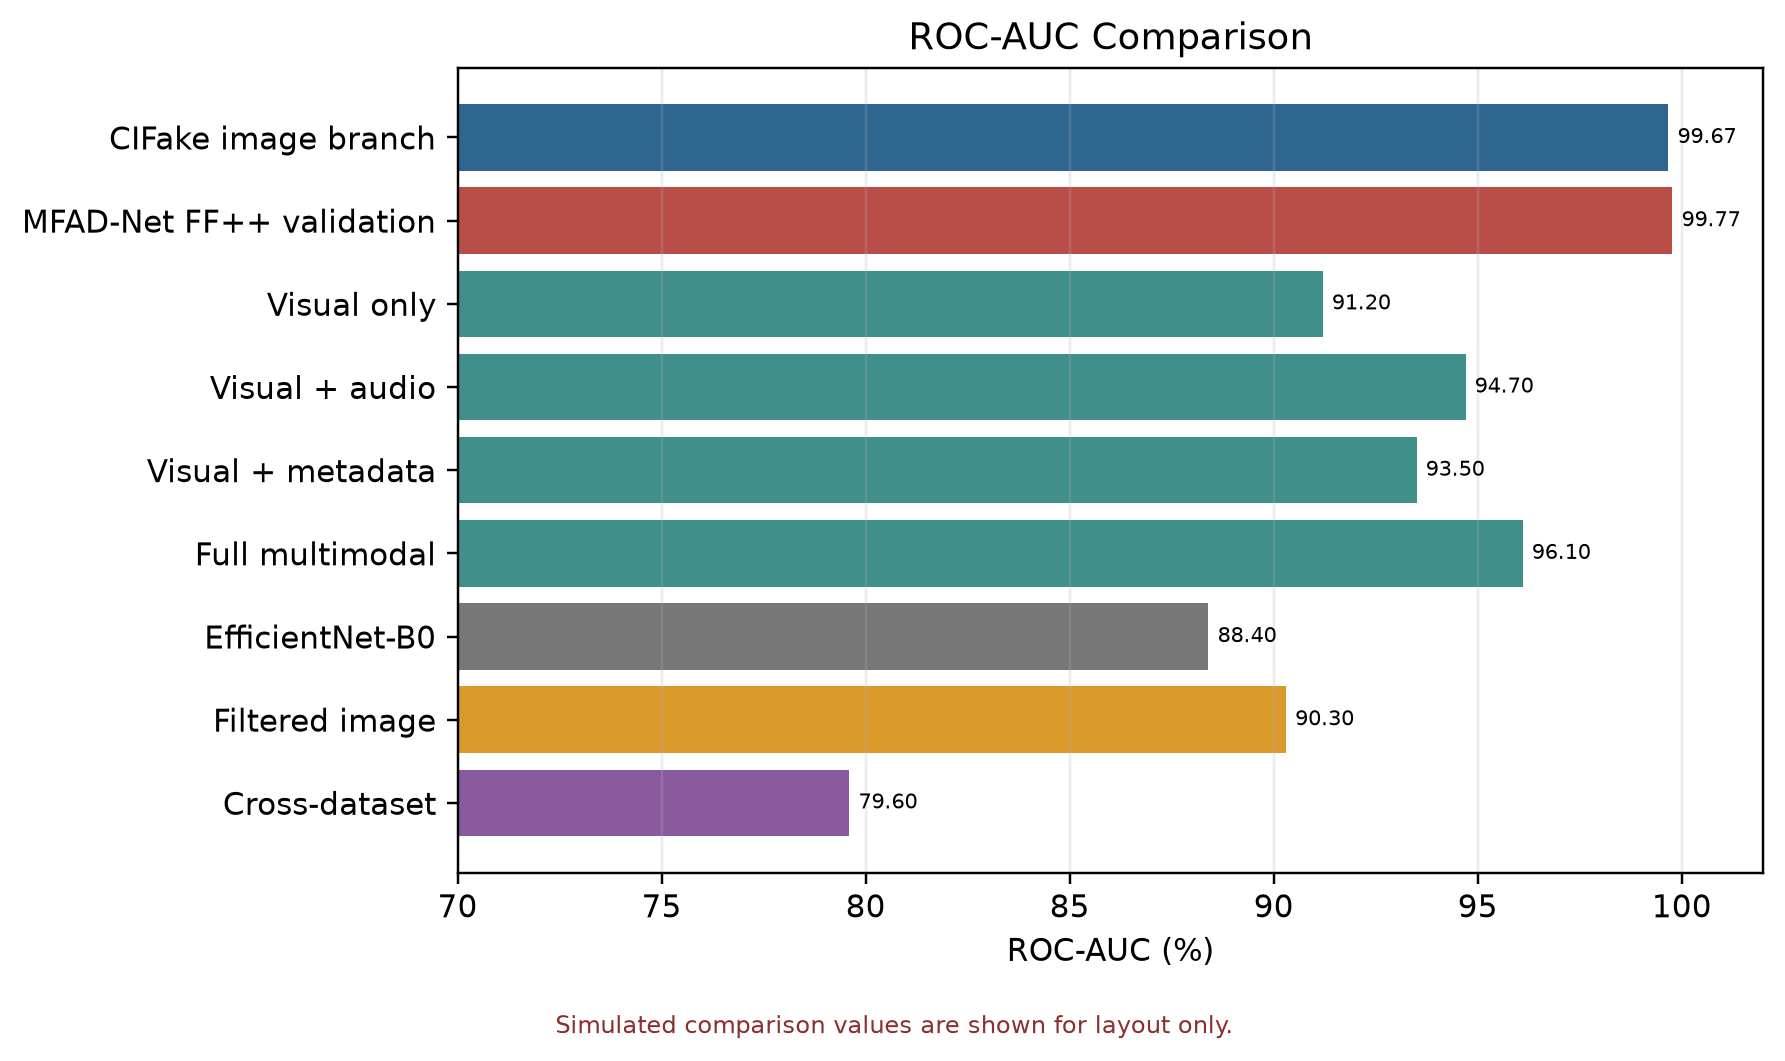
\includegraphics[width=0.98\columnwidth]{figures/simulated_roc_auc.png}
\caption{Illustrative ROC-AUC comparison using simulated values; not experimental results.}
\label{fig:roc_placeholder}
\end{figure}

\subsection{Discussion}

The current results establish that the CIFake image branch can learn a strong decision boundary on its held-out CIFake validation split. This result should be interpreted as in-dataset image classification performance rather than a direct estimate of performance on arbitrary social-media content. The model's use of an FFT branch is motivated by the complementary frequency-domain evidence described in the methodology, while the effect of that branch remains to be isolated through a controlled ablation.

The final comparison will examine whether the multimodal architecture provides an improvement over individual modality configurations. In particular, the contribution of frequency-domain information will be examined by comparing visual-only and visual-frequency configurations, while the contribution of audio, metadata, and temporal signals will be evaluated through ablation experiments. The FaceForensics++ validation result is an initial real-data training result; it does not establish generalization to unseen deepfake sources.

Cross-dataset results will also be considered because performance on a single dataset does not necessarily represent behavior under changing media distributions. Filtered-image experiments are especially relevant to the application because color grading, blur, sharpening, and recompression can alter forensic evidence. The TSDD component will be evaluated separately by measuring the MMD value between the reference and incoming feature distributions.

\begin{figure}[htbp]
\centering
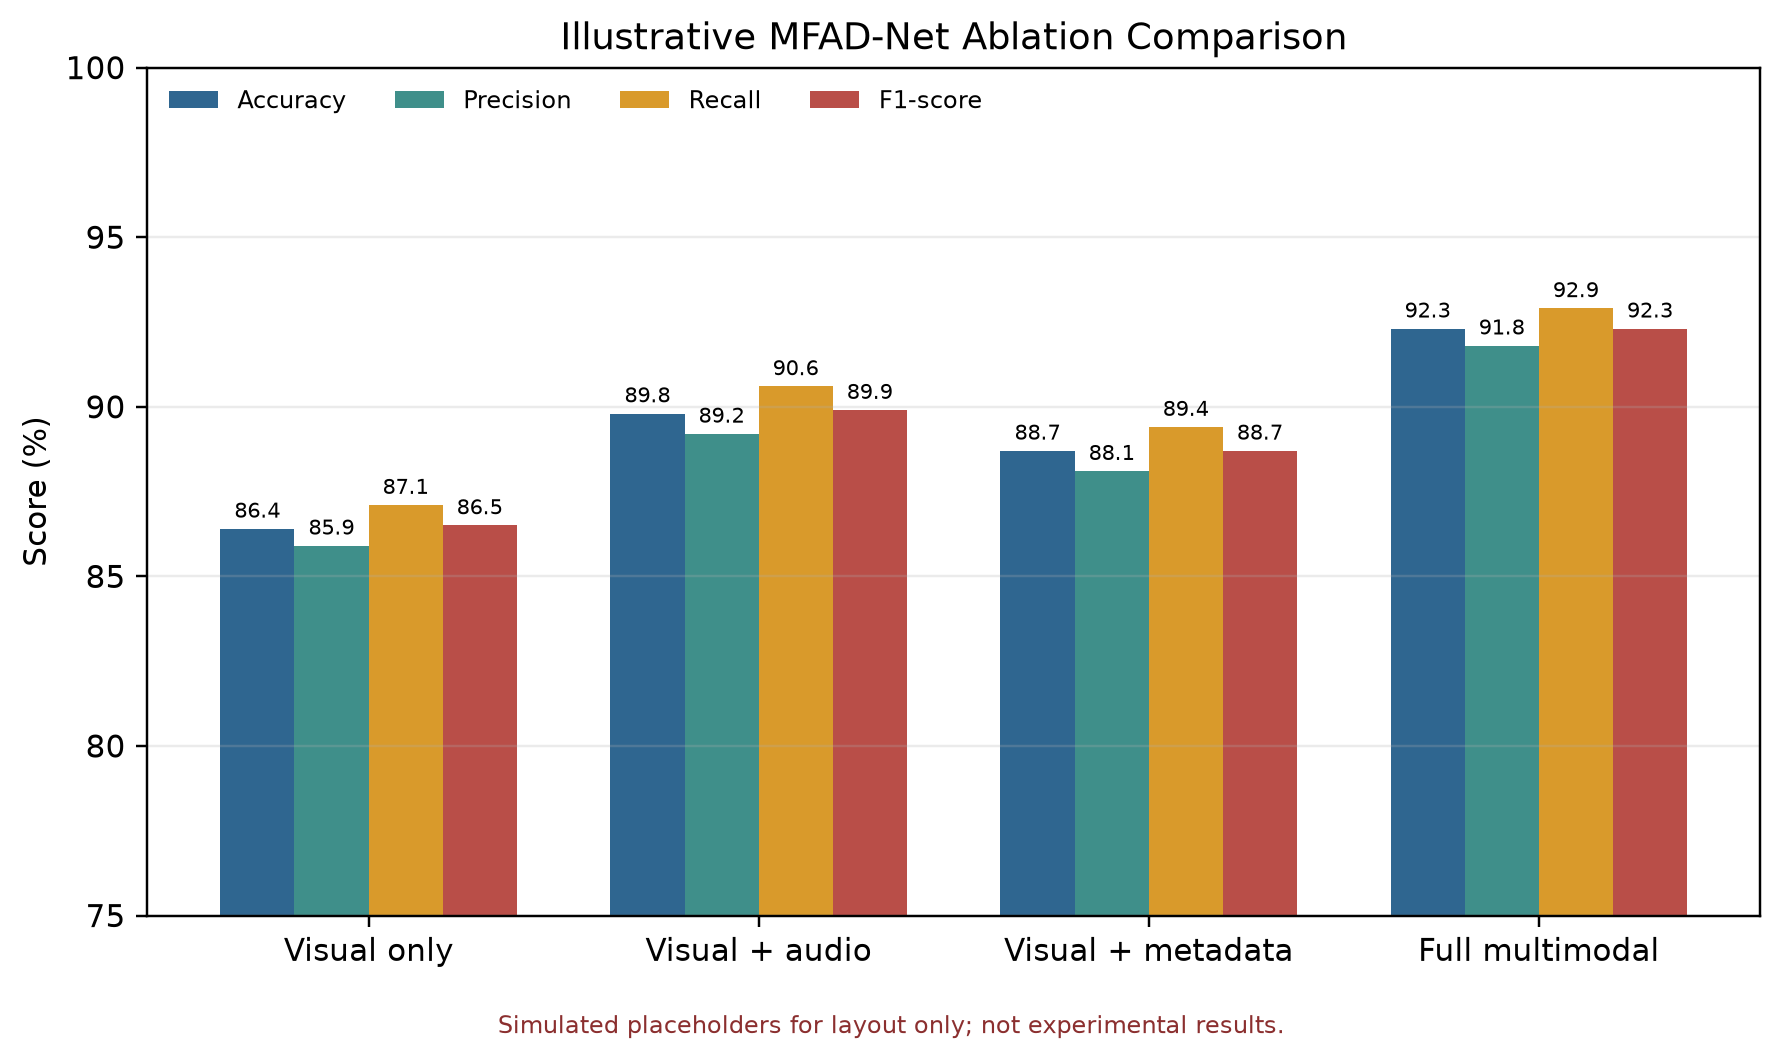
\includegraphics[width=0.98\columnwidth]{figures/simulated_ablation.png}
\caption{Illustrative MFAD-Net ablation comparison using simulated values; not experimental results.}
\label{fig:filtered_placeholder}
\end{figure}

The numerical values currently reported in the tables are limited to recorded project artifacts. The CIFake values come from the latest validation prediction file, and the FaceForensics++ values come from the full multimodal validation checkpoint recorded at epoch 17. Precision, recall, F1-score, and held-out FaceForensics++ test metrics were not recorded for that run. The held-out full multimodal FaceForensics++ test evaluation, filtered-image evaluation, and cross-dataset experiments were not completed in the current study and are marked accordingly rather than assigned numerical values.

\section{Limitations and Future Work}

The current MFAD-Net implementation is a research prototype and has several areas that require further development. The effectiveness of multimodal detection can be affected by the availability and quality of individual modalities. Social-media content may contain compressed video, noisy audio, incomplete metadata, or missing audio streams. Future work will therefore investigate modality-aware processing to improve robustness when individual inputs are degraded or unavailable.

The Temporal-Semantic Drift Detector currently provides a mechanism for identifying changes in incoming feature distributions. However, automatic model adaptation following a detected drift has not yet been completed. Future work will investigate continual-learning strategies that can incorporate newly observed manipulation patterns while reducing the risk of catastrophic forgetting.

The proposed explainability components using Grad-CAM and LIME also require further implementation and evaluation. Future experiments will investigate whether modality-specific explanations can help users understand the evidence contributing to a deepfake prediction.

Further evaluation is also required under realistic social-media conditions, including different compression levels, video resolutions, transcoding operations, noisy audio, and previously unseen manipulation techniques. Cross-dataset experiments will be used to assess whether the proposed multimodal representation generalizes beyond the data used during training.

Finally, the computational cost of multimodal processing will be studied for practical deployment. Model optimization, efficient feature extraction, and asynchronous processing can be explored to reduce inference time while maintaining detection performance.

\section{Conclusion}

This paper presented Social Detect, a multimodal application based on the MFAD-Net design for deepfake detection in social-media environments. The implemented system combines spatial and frequency-domain visual information with heuristic audio, temporal, compression, noise, metadata, and ensemble signals. The MFAD-Net prototype additionally provides audio, metadata, Cross-Modal Attention Fusion, and Temporal-Semantic Drift Detection components for continued experimentation.

The framework is designed as a modular system with a FastAPI backend, dashboard, and browser extension, providing a foundation for practical media analysis and monitoring. The completed CIFake and initial FaceForensics++ validation experiments demonstrate the operation of the primary model paths, while further evaluation is needed under realistic social-media transformations rather than establishing production-level accuracy.

The current system remains under development. Future work will focus on completing ASVspoof 5 audio training, evaluating filtered and cross-dataset inputs, measuring modality ablations, completing adaptive model updating, implementing the proposed explainability components, and optimizing the framework for efficient social-media deployment.

\begin{thebibliography}{00}

\bibitem{sfiad}
Y. Kou, P. Li, H. Ma, J. Zhou, Z. Huang, and X. Li,
``SFIAD: Deepfake detection through spatial-frequency feature integration and dynamic margin optimization,''
\textit{Artificial Intelligence Review},
vol. 58, art. no. 217, 2025,
doi: 10.1007/s10462-025-11225-7.

\bibitem{javed2025av}
M. Javed, Z. Zhang, F. H. Dahri, A. A. Laghari, M. Krajcik, and A. S. Almadhor,
``Audio-visual synchronization and lip movement analysis for real-time deepfake detection,''
\textit{International Journal of Computational Intelligence Systems},
vol. 18, art. no. 170, 2025,
doi: 10.1007/s44196-025-00911-7.

\bibitem{zhang2025continual}
X. Zhang, P. Zhu, C. Zhang, Z. Yan, J. Cheng, M. Lao, S. Cai, and Y. Guo,
``Generalization-Preserved Learning: Closing the Backdoor to Catastrophic Forgetting in Continual Deepfake Detection,''
in \textit{Proc. IEEE/CVF Int. Conf. Comput. Vis. (ICCV)},
2025, pp. 3798--3808.

\bibitem{multimedia_survey_2025}
A. A. Khan, A. A. Laghari, S. A. Inam, S. Ullah, M. Shahzad, and D. Syed,
``A survey on multimedia-enabled deepfake detection: state-of-the-art tools and techniques, emerging trends, current challenges \& limitations, and future directions,''
\textit{Discover Computing},
vol. 28, art. no. 48, 2025,
doi: 10.1007/s10791-025-09550-0.

\bibitem{multimodal_forgery_review_2025}
D. Tan, Y. Yang, C. Niu, S. Li, D. Yang, and B. Tan,
``A review of deep learning based multimodal forgery detection for video and audio,''
\textit{Discover Applied Sciences},
vol. 7, art. no. 987, 2025,
doi: 10.1007/s42452-025-07629-3.

\bibitem{generalization_survey_2026}
H.-H. Nguyen-Le, V.-T. Tran, D.-T. Nguyen, and N.-A. Le-Khac,
``Deepfake detection across image, video, and audio: a comprehensive survey with empirical evaluation of generalization and robustness,''
\textit{Artificial Intelligence Review},
vol. 59, art. no. 203, 2026,
doi: 10.1007/s10462-026-11608-4.

\end{thebibliography}

\end{document}
